\documentclass [xcolor=svgnames, t] {beamer} 
\usepackage[utf8]{inputenc}
\usepackage{booktabs, comment} 
\usepackage[absolute, overlay]{textpos} 
\usepackage{pgfpages}
\usepackage[font=footnotesize]{caption}
\useoutertheme{infolines} 

\AtBeginSection[]{
  \begin{frame}
  \vfill
  \centering
  \begin{beamercolorbox}[sep=8pt,center,shadow=true,rounded=true]{title}
    \usebeamerfont{title}\insertsectionhead\par%
  \end{beamercolorbox}
  \vfill
  \end{frame}
}


%\definecolor{brownbrown}{RGB}{56, 28, 0}
%\definecolor{brownred}{RGB}{228, 0, 43}

%\setbeamercolor{title in head/foot}{bg=brownred, fg=brownbrown}
%\setbeamercolor{author in head/foot}{bg=myuniversity}
\setbeamertemplate{page number in head/foot}{}
\usepackage{csquotes}


\usepackage{amsmath}
\usepackage[makeroom]{cancel}
\usepackage[absolute,overlay]{textpos}

%\usepackage{textpos}

\usepackage{tikz}

\usepackage{media9} 

\usetheme{Madrid}
%\definecolor{myuniversity}{RGB}{56, 28, 0}
%\usecolortheme[named=myuniversity]{structure}
\usepackage{tikz}



\title[Viscosidad]{Clase No.12: Est\'atica de los fluidos}
\subtitle{Dispositivos para medir presi\'on}
\institute[]{Departamento de Ingenier\'ia Civil y Agr\'icola\\ Facultad de Ingenier\'ia  \\Universidad Nacional de Colombia - Sede Bogot\'a}
\titlegraphic{
\includegraphics[height=2.0cm]{escudoUnal.png}}
\author[LAM]{Luis Alejandro Morales \\ \href{https://lamhydro.github.io}{https://lamhydro.github.io}}


%\institute[]{Department of Earth, Environmental, and Planetary Sciences  \\Brown University}
\date{\today}


\addtobeamertemplate{navigation symbols}{}{%
    \usebeamerfont{footline}%
    \usebeamercolor[fg]{footline}%
    \hspace{1em}%
    \insertframenumber/\inserttotalframenumber
}

\begin{document}
\begin{frame}
\maketitle
\end{frame}


%%%%%%%%%%%%%%%%%%%%%%%%%%%%
\logo{\vspace{-0.2cm}
\includegraphics[height=0.8cm]{escudoUnal.png}~%
}
%%%%%%%%%%%%%%%%%%%%%%%%%%



\begin{frame}
\frametitle{Table of Contents}
\tableofcontents
\end{frame}

\section{Bar\'ometro}
\begin{frame}{Bar\'ometro}
\begin{block}{}
El \emph{Bar\'ometro} es un instrumento que sirve para medir la \emph{presi\'on atmosf\'erica}, la cual tambi\'en se conoce como la \emph{presi\'on barom\'etrica}. El Bar\'ometro fue inventado por Evangelista Torricelli entre 1608 y 1647.
\end{block}
\end{frame}

\begin{frame}{Bar\'ometro}
\begin{columns}
\column{0.5\textwidth}
\vspace{-1cm}
\begin{block}{}
El \emph{Bar\'ometro} consiste en invertir un tubo de ensayo lleno de mercurio dentro de un recipiente con mercurio abierto a la atm\'osfera.  La presion en el punto B es igual a la presion atmoferica, mientras la presion en el punto C puede considerarse igual zero. Escribiendo el balance de fuerzas sobre la columna de mercurio:
$$
P = \rho g h
$$
donde $\rho$ es la densidad del mercurio. Note que la altura $h$ de la columns es siempre la misma independiente del diametro del tubo. 
\end{block}
\column{0.5\textwidth}
\begin{textblock*}{6.5cm}(6.8cm,2.3cm) % {block width} (coords)
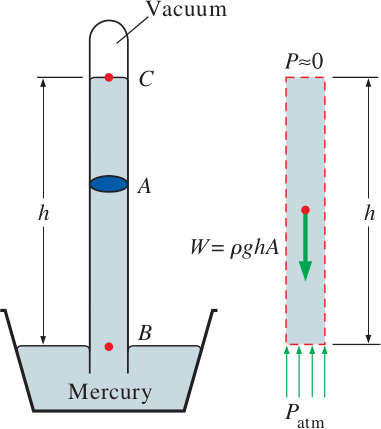
\includegraphics[width=0.9\textwidth]{baro1}
\end{textblock*}
\end{columns}
\end{frame}

\begin{frame}{Bar\'ometro}
\begin{block}{Ideas generales de la $P_{atm}$}
\begin{itemize}
\item La $P_{atm}$ disminuye con la altura. 
\item Si $P_{atm}$ depende del peso del aire arriba de una posicion determinada, esta no solo cambia con la altitud, tambien con las condiciones climaticas.
\item Como la temperatura y la presion disminuyen con la altura, cocinar hervir agua en sitios en altas altitudes toma mayor tiempo.
\item Es comun el sangrado nasal en altas altitudes porque la diferencia entre la presion sanguinea y la presion atmosferica se hace mayor por lo que los vasos sanquineos de la nariz son incapaces de soportar este esfuerzo adicional y terminan rompiendose. 
\item Como en altas altitudes la densidad del aire es mas baja, la cantidad de oxigeno por unidad de volumen es menor, por eso nos cansamos mas rapidamente en estos lugares y experimentamos dificultad al respirar.
\end{itemize}
\end{block}
\end{frame}

\section{Manometr\'ia}
\begin{frame}{Manometr\'ia}
\begin{block}{}
La \emph{manometr\'ia} se define como la medici\'on de presiones (o diferencia de presiones)con base en el desplazamiento de las columnas de fluidos. Los \emph{man\'ometros} son dispositivos que se adaptan a depositos, tuberias o canales con el proposito de medir presiones de fluidos en reposo o en movimiento. El c\'alculo de la presi\'on se hace con base en la ecuaci\'on fundalmental de la est\'atica de fluidos y los datos que registra el man\'ometro.
Existen dos tipos de dispositivos para medir presi\'on manom\'etrica:
\begin{itemize}
\item Tubos piezom\'etricos
\item Man\'ometros 
\end{itemize}  
\end{block}
\end{frame}

\begin{frame}{Manometr\'ia}
\footnotesize
\vspace{-0.5cm}
\begin{block}{¿Como resolver problemas con manometros?}
Recuerde que para resolver cualquier problema de manometros:
\begin{enumerate}
\item El cambio de presi\'on en una columna de fluido $h$ es: $\Delta P = \gamma h$.
\item La presi\'on en un fluido incrementa hacia abajo y disminuye hacia arriba ($P_{down} > P_{top}$).
\item Dos puntos conectados por un fluido continuo en reposo sobre el mismo plano horizontal tienen la misma presi\'on. 
\end{enumerate}
\end{block}
\begin{columns}
\column{0.65\textwidth}
Cuando existen differentes tipos de fluidos conectados continuamente y en reposo se puede calcular la presi\'on en un punto determinado partiendo del punto cuya presi\'on es conocida e ir adicionando o substrayendo el termino $\gamma h$ en la direcci\'on al punto de presi\'on desconocida. 
%Por ejemplo si tenemos los fluidos de la figura y queremos calcular la presion en el punto 1, empezamos desde la presion conocida $P_{atm}$ y vamos avanzando hasta el punto 1, lo cual da: 
$$
P_{atm} + \gamma_1 h_1 + \gamma_2 h_2 + \gamma_3 h_3 = P_1
$$
En el caso en que los tres fluidos tuvieran la misma densidad, la ecuaci\'on anterior quedar\'ia: 
$$
P_{atm}+\gamma (h_1 + h_2 + h_3) = P_1
$$
\column{0.35\textwidth}
% Fig 3.21 Cengel
%\begin{figure}[h]
%\centering
\begin{textblock*}{4.5cm}(9.0cm,4.7cm) % {block width} (coords)
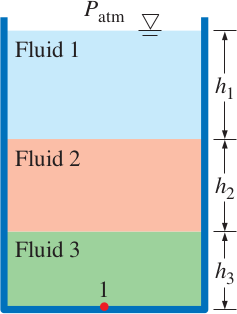
\includegraphics[width=0.6\textwidth]{mano3}
\end{textblock*}
%\caption{Tres tipos de fluido en reposo de diferente $\rho$ ubicados unos sobre el otro.}
%\label{mano3}
%\end{figure}
\end{columns}

\end{frame}

\subsection{Tubos piezom\'etricos}
\begin{frame}{Tubos piezom\'etricos}
\begin{block}{}
Los \emph{piezometros} son dispositivos elementales para medir presi\'on. Consiste en un tubo que se conecta por su extremo inferior al recipiente que contiene el l\'iquido cuya presi\'on se quiere medir. El l\'iquido del recipiente llena parcialmente el tubo hasta alcanzar un nivel B.
\end{block}
\begin{columns}
\column{0.6\textwidth}
Presi\'on absoluta en A:
$$
P_A = P_{atm}+\gamma h
$$
Presi\'on relativa en A ($P_{atm}=0$):
$$
P_{rA} = \gamma h
$$
\column{0.4\textwidth}
\begin{textblock*}{5.5cm}(6.0cm,5.3cm) % {block width} (coords)
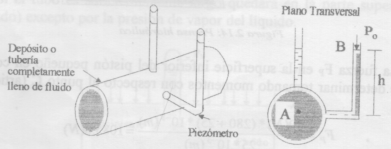
\includegraphics[width=1.2\textwidth]{piezo}
\end{textblock*}
% Figura 2.15 (Duarte)
\end{columns}
\end{frame}

\begin{frame}{Tubos piezom\'etricos}
\begin{columns}
\column{0.5\textwidth}
Para el caso en que la presi\'on del liquido es menor que $P_{atm}$ (e.g. cavitaci\'on en tuber\'ias), el tubo piezom\'etrico deber\'a tener la siguiente forma:
\begin{textblock*}{5.5cm}(0.5cm,4.3cm) % {block width} (coords)
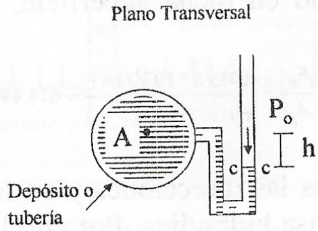
\includegraphics[width=\textwidth]{mano216}
\end{textblock*}
% Figura 2.16 (Duarte)
\column{0.5\textwidth}
Presi\'on absoluta en A:
$$
P_A = P_{atm}-\gamma h
$$
Presi\'on relativa en A ($P_{atm}=0$):
$$
P_{rA} = -\gamma h
$$
Los piez\'ometros son utilizados para medir bajas presiones, de lo contrario el tubo deber\'ia ser muy largo. 
\end{columns}
\end{frame}


\subsection{Man\'ometros}
\begin{frame}{Man\'ometros}
\begin{block}{}
%Definicio
Los \emph{manometros} son dispositivos utilizados para medir presiones altas. Contienen l\'iquidos de peso espec\'ifio elevado con el fin de evitar que la columna manom\'etrica alcance alturas elevadas. En general, existen tres tipos de man\'ometros:
\begin{itemize}
\item Manometro abierto
\item Manometro diferencial
\item Manometro diferencial compuesto
\end{itemize}
\end{block}
\end{frame}


\begin{frame}{Man\'ometros abiertos}
\vspace{-0.5cm}
\small
\begin{block}{}
Estos man\'ometros son llenados parcialmente con \emph{mercurio} el cual tiene un peso espec\'ifico $\approx$ 15 veces mas que el agua. 
\end{block}
\begin{itemize}
\item $P\ >\ P_{atm}$
\begin{columns}
\column{0.5\textwidth}
En el man\'ometro de la figura, el mercurio ocupa la zona BCD del tubo, donde la $P_{atm}$ actua en D. La presi\'on en A es:
$$
P_A = P_{atm}+\gamma_{Hg}h - \gamma h_1
$$
Note que $P_B = P_C$ (B y C en el mismo plano horiozontal).
\column{0.5\textwidth}
\begin{textblock*}{4.5cm}(8.0cm,2.3cm) % {block width} (coords)
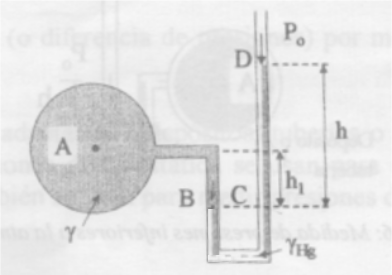
\includegraphics[width=\textwidth]{manome1}
\end{textblock*}
%Figura 2.17 (Duarte)
\end{columns}
\item $P\ <\ P_{atm}$
\begin{columns}
\column{0.5\textwidth}
De acuerdo con la figura, la presi\'on A es:
$$
P_A = P_{atm}-\gamma_{Hg}h - \gamma h_1
$$
Note que $P_D = P_{atm}$ y que $P_C = P_D$.
\column{0.5\textwidth}
\begin{textblock*}{4.5cm}(8.0cm,5.3cm) % {block width} (coords)
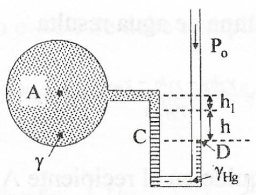
\includegraphics[width=\textwidth]{mano218}
\end{textblock*}
%Figura 2.18 (Duarte)
\end{columns}
\end{itemize}
\end{frame}


\begin{frame}{Man\'ometros diferenciales}
\vspace{-0.5cm}
\begin{block}{}
\begin{columns}
\column{0.6\textwidth}
Estos dispositivos, como su nombre lo indica, se utilizan para determinar diferencias de presi\'on en donde el(los) $\gamma$ de los liquidos deben ser mayores al $\gamma$ del sistema e inmisibles. Para establecer la presi\'on entre A y E, se procede siguiendo los siguientes pasos
\column{0.4\textwidth}
\begin{textblock*}{4.5cm}(7.7cm,1.0cm) % {block width} (coords)
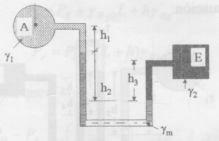
\includegraphics[width=\textwidth]{manome2}
\end{textblock*}
%Figura 2.19 (Duarte)
\end{columns}
\end{block}
\begin{enumerate}
\item Comenzando por un extremo (A o E), anotar la presi\'on (en unidades adecuadas).
\item Se suma a este valor, el cambio de presi\'on que se tenga de un menisco al siguiente: $+$ si el segundo menisco se encuentra a menor elevaci\'on, $-$ si est\'a a mayor elevaci\'on.
\item Se procede de esta manera hasta alcanzar la presion en el otro extremo (E). El resultado se igua a la presi\'on en E (se conozca o no).
\item Se despeja al presi\'on o diferencia de presiones desconocida de la ecuaci\'on. 
\end{enumerate}
\end{frame}

\begin{frame}{Man\'ometros diferenciales}
\begin{columns}
\column{0.6\textwidth}
De acuerdo con los pasos anteriores, para el caso del man\'ometro de la figura, se tendr\'a que:
$$
P_A + \gamma_1 h_1 + \gamma_m h_2 - \gamma_2 h_3 = P_E
$$
La diferencia de presiones en columna de agua es:
$$
\frac{P_A - P_E}{\gamma_{H_2 O}} = \frac{\gamma_2 h_3 - \gamma_1 h_1 - \gamma_m h_2}{\gamma_{H_2 O}} = S_2 h_3 - S_1 h_1 - S_m h_2
$$
\column{0.4\textwidth}
\begin{textblock*}{5.0cm}(7.5cm,1.8cm) % {block width} (coords)
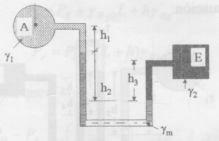
\includegraphics[width=\textwidth]{manome2}
\end{textblock*}
%Figura 2.19 (Duarte)
\end{columns}
\vspace{0.5cm}
donde:
\begin{itemize}
\item[$S_1$]: Gravedad espec\'ifica del l\'iquido en el recipiente A.
\item[$S_2$]: Gravedad espec\'ifica del l\'iquido en el recipiente E.
\item[$S_m$]: Gravedad espec\'ifica del l\'iquido manom\'etrico.
\end{itemize}
\end{frame}

\begin{frame}{Man\'ometros diferenciales}
\vspace{-0.4cm}
\begin{columns}
\column{0.6\textwidth}
Los man\'ometros pueden ser conectados entre dos secciones de una misma tuber\'ia  que transporta l\'iquido o gas cuyo peso espec\'ifico es $\gamma_1$. La diferencia de presi\'on $P_1 - P_2$ partiendo de $1$ es:
$$
P_1 + \gamma_1 (a+h) - \gamma_2 h - \gamma_1 a = P_2
$$
\vspace{0.5cm}
\column{0.4\textwidth}
\begin{textblock*}{4.5cm}(8cm,1cm) % {block width} (coords)
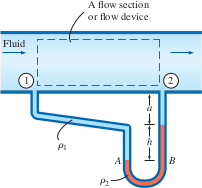
\includegraphics[width=\textwidth]{mano4}
\end{textblock*}
\end{columns}
Note que los puntos a una distancia $a$ tienen una misma presi\'on por estar al mismo nivel en el manometro, simplificando:
$$
P_1 - P_2 = (\gamma_2 - \gamma_1)h
$$
Si el fluido que fluye a lo largo de la tuberia es gas, $\gamma_1 \ll \gamma_2$ por lo que la ecuacion anterior se convierte en $P_1-P_2 \cong \gamma_2 h$.
\end{frame}

\begin{frame}{Man\'ometros diferenciales compuestos}
%\vspace{-0.5cm}
\begin{columns}
\column{0.6\textwidth}
Cuando la diferencia de presi\'on es apreciable, se pueden usar man\'ometros diferenciales con diferentes l\'iquidos como se muestra en la figura. Siguiendo el procedimiento anterior, la suma de presiones es:
\column{0.4\textwidth}
\begin{textblock*}{7.5cm}(7.5cm,1.0cm) % {block width} (coords)
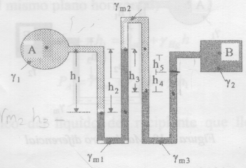
\includegraphics[width=0.7\textwidth]{manome3}
\end{textblock*}
%Figura 2.20 (Duarte)
\end{columns}
\vspace{1cm}
$$
P_A + \gamma_1 h_1 - \gamma_{m1} h_2 + \gamma_{m2} h_3 - \gamma_{m3} h_4 - \gamma_2 h_5 = P_B
$$
 
$$
P_A - P_B = -\gamma_1 h_1 + \gamma_{m1} h_2 - \gamma_{m2} h_3 + \gamma_{m3} h_4 + \gamma_2 h_5
$$

La diferencia de presi\'on entre A y B es:
$$
\frac{ P_A - P_B }{\gamma_{H_2 0}} = -S_1 h_1 + S_{m1} h_2 - S_{m2} h_3 + S_{m3} h_4 + S_2 h_5
$$

\end{frame}
\end{document}

